% Extracted from maximumsAndMinimums.tex, problem #8
\begin{problem}
Sketch a possible graph of a function $f$ that has the following properties:\\
	\begin{enumerate}
		\item $f$ is defined on the interval $(0,6)$.
		\item $f$ has no local maximums.
		\item $f$ has exactly two local minimums.
	\end{enumerate}
\WkstHop
	
		\begin{freeResponse}
		This could be the graph of $f$. Notice two local minimums: at $x=2$ and at $x=4$.
		%\begin{image}
		%\includegraphics{Figure 21.pdf}
		%\end{image}
			\begin{center}
					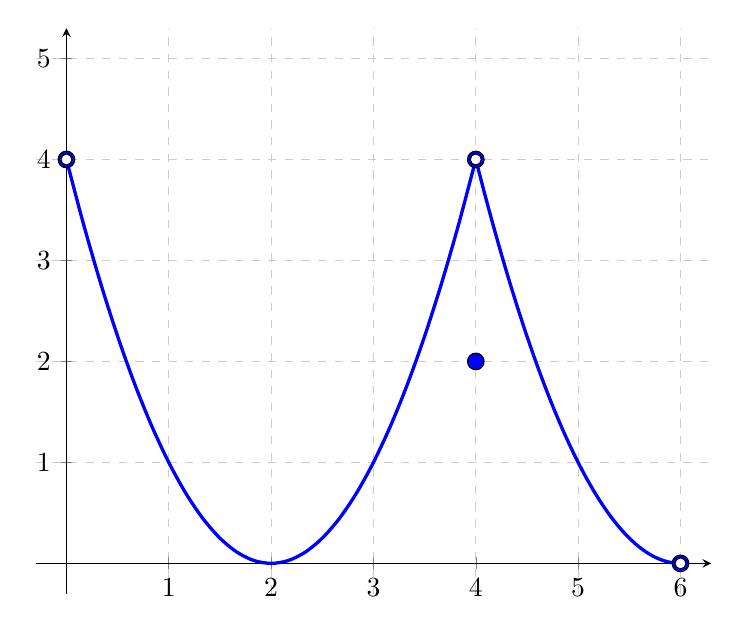
\begin{tikzpicture}
						\begin{axis}[
							xmin=-0.3, xmax=6.3, ymin=-0.3,ymax=5.3,    
							axis lines =middle, 
							every axis y label/.style={at=(current axis.above origin),anchor=south},
							every axis x label/.style={at=(current axis.right of origin),anchor=west},
							xtick={0,...,6}, ytick={0,...,5},
							grid=major, width=4in,
							grid style={dashed, gray!40} 
							]
							\addplot[color=blue, very thick, smooth, domain=0:4]{(x-2)^2};
							\addplot[color=blue, very thick, smooth, domain=4:6]{(x-6)^2};

							\draw[fill=blue] (axis cs:0,4) circle [color=blue,radius=3pt] node [below right] {};
							\draw[fill=white] (axis cs:0,4) circle [color=white,radius=2pt] node [below right] {};
							\draw[fill=blue] (axis cs:4,4) circle [color=blue,radius=3pt] node [below right] {};
							\draw[fill=white] (axis cs:4,4) circle [color=white,radius=2pt] node [below right] {};
						
							
							\draw[fill=blue] (axis cs:6,0) circle [color=blue,radius=3pt] node [below right] {};
							\draw[fill=white] (axis cs:6,0) circle [color=white,radius=2pt] node [below right] {};
							\draw[fill=blue] (axis cs:4,2) circle [color=blue,radius=3pt] node [below right] {};
						
						
						
						\end{axis}
					\end{tikzpicture}
				\end{center}

		\end{freeResponse}	
		
\end{problem}
